\documentclass[12pt,a4paper]{report}
\usepackage[utf8]{inputenc}
\usepackage{amsfonts}
\usepackage{setspace}
\usepackage{graphicx}
\usepackage{array}
\usepackage{fancyhdr}
\usepackage{geometry}
\usepackage{ragged2e}
\usepackage{color}
\usepackage{tabularx}
\usepackage[backend=biber, sorting=none, style=ieee]{biblatex}
\usepackage{color}

\addbibresource{reference.bib}
\geometry{
a4paper,
total={210mm,297mm},
left=1.0in,
right=0.85in,
top=0.65in,
bottom=0.65in,
}
\begin{document}
\pagestyle{empty}
\begin{center}

  {\large \textbf{Visvesvaraya Technological University, Belagavi – 590018}}
  \begin{figure}[hbtp]
    \centering
    
\includegraphics[width=2.3cm,height=3cm]{./pic/vtu}
  \end{figure}
 
  \textbf{PROJECT WORK DESIGN PHASE REPORT}
  \par
  \textbf{ON}
  \par
  \vspace{6pt}
  {\Large \textbf{Cloud-Based Smart Monitoring System for Baby Health and Safety}}
  \par
  \vspace{12pt}
  \par
  \textit{\textbf{Submitted in partial fulfillment of the requirements for the degree }}
  \par
  \vspace{12pt}
  \large \textbf{BACHELOR OF ENGINEERING }
  \par
  \textbf{in}
  \par
  \large \textbf{COMPUTER SCIENCE \& ENGINEERING}
  \par
  \vspace{12pt}
  \textit{\textbf{Submitted by}}
  \vspace{8pt}

  \begin{center}
    \begin{tabular}{l@{\hspace{2cm}}r}
      \textbf{\large Aaron Tauro}       & \textbf{4SO21CS002} \\
      \textbf{\large Abhik L Salian}    & \textbf{4SO21CS004} \\
      \textbf{\large Akhil Shetty M}    & \textbf{4SO21CS013} \\
      \textbf{\large H Karthik P Nayak} & \textbf{4SO21CS058} \\
    \end{tabular}
  \end{center}

  \vspace{12pt}
  \textit{\textbf{Under the Guidance of}}
  \par
  \vspace{6pt}
  \textbf{Dr Sridevi Saralaya}
  \par
  \vspace{2pt}
  \normalsize { Professor, Department of CSE }
  \par
  \begin{figure}[hbtp]
    \centering
    
\includegraphics[scale=0.6]{./pic/sjeclogo}
  \end{figure}
  \large \textbf{DEPT. OF COMPUTER SCIENCE AND ENGINEERING}
  \par \Large \textbf{ST JOSEPH ENGINEERING COLLEGE}
  \par
  \textbf{An Autonomous Institution}
  \par
  {\large{(Affiliated to VTU Belagavi, Recognized by AICTE, Accredited by NBA)}}
  \par
  \vspace{3pt}
  {\large \textbf{Vamanjoor, Mangaluru - 575028, Karnataka}}
  \par
  \vspace{12pt}
  {\Large \textbf{2024-25}}
\end{center}

\newpage

%%%%%%%%%%%%%%%%%%%%%%%%%% Acknowledgement %%%%%%%%%%%%%%%

% \pagestyle{empty}
% \setstretch{1.8}
% \pagenumbering{roman}
% \chapter*{\centering ACKNOWLEDGEMENT}


% The joy and satisfaction that accompany the partial completion of any task would be incomplete without thanking those who made it possible. We consider ourselves proud to be a part of St Joseph Engineering College, the institution which moulded us in all our endeavours. We express our sincere gratitude to the management for providing state-of-the-art facilities and support throughout our project.
% \vspace{10pt}\\
% We owe our profound gratitude to our project guide \textbf{Dr Sridevi Saralaya}, Professor and Head of the Department, Computer Science and Engineering, St Joseph Engineering College, for her valuable guidance and support during the entire period of our project.
% \vspace{10pt}\\
% We are indebted to our respected Principal, \textbf{Dr Rio D'Souza} for his valuable guidance and encouragement throughout the project.
% \vspace{10pt}\\
% We express our sincere gratitude to \textbf{Rev Fr Wilfred Prakash D'Souza}, Director, and \textbf{Rev Fr Kenneth Rayner Crasta}, Assistant Director, for their unwavering support and provision of facilities throughout the development stages of our project.
% \vspace{10pt}\\
% We wish to express our sincere gratitude to all the Faculty and Technical staff of the Department and friends and family for their valuable help and support during the period of development of our project .\\

% \newpage

%%%%%%%%%%%%%%%%%%%%%%%%%% Abstract %%%%%%%%%%%%%%%
\pagestyle{empty}
\setstretch{1.5}

\chapter*{\centering ABSTRACT}

\begin{justify}

  The need for reliable infant monitoring systems has become increasingly essential due to the high demands of modern parenting and the need to ensure infant safety. This project presents a ``Cloud-Based Smart Monitoring System for Baby Health and Safety," designed to monitor various health metrics of infants, such as body temperature, heart rate, room temperature, humidity, and posture, offering parents peace of mind through real-time notifications and alerts.

\noindent Research and development in the field of non-contact health monitoring have progressed significantly, utilizing technologies like remote photoplethysmography and computer vision for health parameter detection. However, most current systems either lack comprehensive monitoring capabilities or depend on contact-based sensors that may disrupt infant comfort. This project addresses these limitations by proposing a comprehensive, non-contact monitoring solution that integrates contactless sensors and machine learning techniques to monitor critical parameters. Our goal is to deliver a holistic, efficient, and user-friendly system for infant health and safety monitoring.

\noindent The research methodology encompasses the development of a mobile application that interacts with a cloud-based system and sensors, designed to monitor and analyze infant health data in real-time. The novel solution incorporates computer vision algorithms to track baby posture and detect when the infant is sleeping on its tummy, potentially preventing sudden infant death syndrome (SIDS). Experimental results demonstrate the reliability and accuracy of the system in various environmental conditions, providing immediate alerts during abnormalities.

\noindent This work demonstrates significant benefits by enhancing infant safety, reducing the need for continuous parental monitoring, and offering peace of mind. The system's cloud-based architecture enables remote monitoring, which saves on resources and energy.

\noindent Future work can explore extending the system’s capabilities to detect additional health parameters and integrate AI for predictive health analysis, making it an even more comprehensive monitoring tool.
  \end{justify}

\setstretch{1.2}
\renewcommand{\contentsname}{\centering Table of Contents}
\tableofcontents

\newpage
\listoftables

\listoffigures








%%%%%%%%%%%%%%%%%%%%% Headders and Footers %%%%%%%%%%%%%%%
\fancyhf{} % clear header and footer
\fancyhead[L]{Cloud-Based Smart Monitoring System for Baby Health and Safety} % header centered
\fancyfoot[L]{Department of Computer Science and Engineering, SJEC, Mangaluru} % footer centered
\fancyfoot[R]{\thepage} % page number on the right
\renewcommand{\headrule}{%
  {\color[RGB]{0,0,0}\hrule width\headwidth height 2pt} % Top line
  \vspace{0.07\baselineskip}% Add space between lines
  {\color[RGB]{0,0,0}\hrule width\headwidth height 0.5pt} % Bottom line
}
\renewcommand{\footrule}{%

  {\color[RGB]{0,0,0}\hrule width\headwidth height 0.5pt} % Top line
  \vspace{0.07\baselineskip}% Add space between lines
  {\color[RGB]{0,0,0}\hrule width\headwidth height 2pt} % Bottom line
}


\renewcommand{\baselinestretch}{1.5}

% \pagestyle{fancy}
% \fancyhf{}
% \lhead{\fontsize{10}{12} \selectfont Bidirectional Communication System for Deaf-blind Individuals}
% \rhead{\fontsize{10}{12} \selectfont Chapter \thechapter}
% \lfoot{\fontsize{10}{12} \selectfont Department of Computer Science and Engineering, SJEC, Mangaluru}
% \rfoot{\fontsize{10}{12} \selectfont Page \thepage}
% \renewcommand{\headrulewidth}{0.5pt}
% \renewcommand{\footrulewidth}{0.5pt}


%%%%%%%%%%%%%%%%%%%%%%% CHapetr 1 Introduction %%%%%%%%%%%%%
\clearpage
\setcounter{page}{1}
\pagestyle{fancy}
\setstretch{1.2}
\pagenumbering{arabic}

\chapter{Introduction}
\par
\section{Background}
The health and safety of infants are critical concerns for parents, particularly when they are unable to provide constant supervision due to other responsibilities. One of the major risks to infants during sleep is Sudden Infant Death Syndrome (SIDS), which can occur if the baby unknowingly assumes an unsafe sleeping posture. In addition to posture, environmental factors like temperature, humidity, and the baby’s health indicators—such as body temperature and heart rate—can have significant impacts on the baby’s well-being. The lack of real-time, comprehensive monitoring systems makes it difficult for parents to detect these risks in time. This project, Cloud-Based Smart Monitoring System for Baby Health and Safety, is designed to bridge this gap by leveraging advanced software algorithms and cloud-based solutions to provide real-time monitoring of a baby’s health and surroundings. With the integration of multiple sensors and a camera, the system ensures that any abnormalities, such as unsafe sleeping postures or sudden health changes, are detected and immediately communicated to the parents through a mobile application, helping to prevent potential health risks.

With the advancement of technology, there has been a growing interest in creating smart monitoring systems that go beyond simple video surveillance, incorporating health data analytics. This project aims to build on existing systems by introducing an innovative, software-focused approach that can simultaneously monitor and process multiple parameters, such as the baby’s posture, heart rate, and environmental conditions. Using cloud computing for real-time data processing and alerts, the system will allow parents to track their child’s well-being from any location, ensuring both the baby’s safety and the parents’ peace of mind. The focus on cloud infrastructure also allows scalability, enabling the system to be expanded with additional features and updates as needed.

\section{Problem statement }
To develop a cloud-based smart monitoring system that addresses the challenges parents face in continuously monitoring their infants, particularly when away from home. The system will use real-time data from sensors and video feeds to detect unsafe sleeping postures, abnormal body temperature, irregular heart rate, and environmental factors such as humidity. By using software-driven algorithms for analysis and alerting, the system will notify parents instantly of any concerns, thus preventing risks like Sudden Infant Death Syndrome (SIDS) and ensuring the infant's health and safety.
\section{Objectives}
The objectives of the proposed project work are:
\begin{enumerate}
    \item To develop a mobile app that collects the body temperature of the baby and room temperature from the cloud, which is transmitted from the monitoring device.
    \item To integrate computer vision technology to detect unsafe sleeping positions of the baby.
    \item To create a user-friendly interface that allows parents to easily monitor real-time temperature readings.
    \item To deliver actionable notifications through app alerts when abnormal readings or unsafe sleeping position is detected.
\end{enumerate}
\section{Scope and Importance of the Project}
The Cloud-Based Smart Monitoring System for Baby Health and Safety aims to provide a comprehensive, software-driven solution for real-time monitoring of a baby’s health, environment, and movements. The project’s scope includes the development of advanced algorithms to detect unsafe sleeping postures using computer vision, as well as the integration of sensor data from temperature, humidity, and heart rate monitors. The software will process this data in real-time through a cloud infrastructure, delivering instant alerts to parents via a mobile application whenever abnormalities are detected, such as a sudden change in the baby’s sleeping position, body temperature, or crying. This monitoring will be continuous and remote, ensuring that parents receive timely notifications even when they are away from home.

The project is highly relevant in today's fast-paced world, where parents are often unable to supervise their children around the clock. The system can be applied in homes, daycares, or hospitals, giving caregivers real-time insight into the baby’s well-being. By focusing on software for analyzing health and environmental data, this project addresses a significant gap in traditional baby monitors, which are often limited in functionality. The use of cloud technology ensures scalability, allowing for future enhancements such as the addition of more sensors or features, thereby making the system adaptable to evolving needs in infant care and monitoring.

%---------------------------- Chapter TWO --------------------------

\chapter{Literature Survey}

\section{IoT Based Smart Baby Monitoring System with Emotion Recognition Using Machine Learning}

\textbf{Identified Problem: }This paper addresses the challenges faced by working parents in continuously monitoring their babies, particularly regarding environmental conditions and emotional states\cite{alam2023iot}.
\setlength{\parskip}{1em}  % Adds 1em space between paragraphs

\noindent\textbf{Methodology:} The authors propose an IoT-based system that integrates various sensors to monitor room temperature, humidity, and emotional recognition through facial detection. Data is transmitted to the Blynk server, allowing real-time monitoring via a mobile application.
\setlength{\parskip}{1em}  % Adds 1em space between paragraphs

\noindent\textbf{Implementation:} The system employs a combination of IoT sensors and machine learning algorithms to detect a baby's cry and facial emotions. Notifications are sent to parents if abnormal conditions are detected.
\setlength{\parskip}{1em}  % Adds 1em space between paragraphs

\noindent\textbf{Results:} The implementation demonstrated effective monitoring capabilities, allowing parents to manage their time efficiently while ensuring their child's well-being.
\setlength{\parskip}{1em}  % Adds 1em space between paragraphs

\noindent\textbf{Inference from Results:} The system significantly alleviates the burden on parents by providing timely notifications and insights into their child's emotional state.
\setlength{\parskip}{1em}  % Adds 1em space between paragraphs

\noindent\textbf{Limitations/Future Scope:} While the system shows promise, it requires further development in terms of data security and privacy, as well as enhancing the accuracy of emotion recognition algorithms
\setlength{\parskip}{1em}  % Adds 1em space between paragraphs

\section{IOT Based Baby Monitoring System}
\textbf{Identified Problem: } This research focuses on creating an efficient and cost-effective monitoring system for infants that can operate in real-time\cite{Singh2021}.

\setlength{\parskip}{1em}  % Adds 1em space between paragraphs

\noindent\textbf{Methodology:}The authors utilize NodeMCU as the main control unit, integrating various sensors to monitor temperature, humidity, and crying. Data is uploaded to the AdaFruit BLYNK server for remote access.
\setlength{\parskip}{1em}  % Adds 1em space between paragraphs

\noindent\textbf{Implementation:}A prototype was developed that includes features like automatic cradle swaying when a baby cries and live video surveillance through an external webcam.
\setlength{\parskip}{1em}  % Adds 1em space between paragraphs

\noindent\textbf{Results:}The prototype proved effective in monitoring vital parameters, demonstrating simplicity and cost-effectiveness.

\setlength{\parskip}{1em}  % Adds 1em space between paragraphs

\noindent\textbf{Inference from Results:} The system's design allows for easy implementation in various settings, making it accessible for many families.
\setlength{\parskip}{1em}  % Adds 1em space between paragraphs

\noindent\textbf{Limitations/Future Scope:} Future improvements could focus on enhancing sensor accuracy and expanding functionalities to include more health parameters.
\setlength{\parskip}{1em}  % Adds 1em space between paragraphs

\section{Internet of Things in Pregnancy Care Coordination and Management}

\textbf{Identified Problem: }This systematic review highlights gaps in existing literature regarding IoT applications in pregnancy and neonatal care\cite{Hossain2023}.
\setlength{\parskip}{1em}  % Adds 1em space between paragraphs


\noindent\textbf{Methodology:} The authors conducted a thorough review of IoT systems used in healthcare, focusing on their application in monitoring pregnant women and newborns.
\setlength{\parskip}{1em}  % Adds 1em space between paragraphs


\noindent\textbf{Implementation:} The review synthesizes findings from various studies to identify trends and challenges in IoT applications for maternal and infant health.
\setlength{\parskip}{1em}  % Adds 1em space between paragraphs

\noindent\textbf{Results:}  It emphasizes the growing importance of IoT in healthcare but also points out significant limitations related to data security and sensor accuracy.
\setlength{\parskip}{1em}  % Adds 1em space between paragraphs


\noindent\textbf{Inference from Results:}  The findings suggest that while IoT has transformative potential in healthcare, there are critical gaps that need addressing for effective implementation.

\setlength{\parskip}{1em}  % Adds 1em space between paragraphs

\noindent\textbf{Limitations/Future Scope:} Future research should focus on improving security protocols and enhancing user experience with IoT devices.

\setlength{\parskip}{1em}  % Adds 1em space between paragraphs


\section{Development of an IoT based Smart Baby Monitoring System with Face Recognition}
\textbf{Identified Problem: }This study tackles the issue of parental anxiety regarding infant safety by proposing an advanced monitoring system\cite{9454187}.
\setlength{\parskip}{1em}  % Adds 1em space between paragraphs


\noindent\textbf{Methodology:} The authors developed a system that combines face recognition technology with environmental monitoring sensors to provide comprehensive oversight of infants' conditions.

\setlength{\parskip}{1em}  % Adds 1em space between paragraphs


\noindent\textbf{Implementation:} The system utilizes machine learning algorithms for face recognition alongside traditional environmental sensors for temperature and humidity monitoring.

\setlength{\parskip}{1em}  % Adds 1em space between paragraphs

\noindent\textbf{Results:}  The proposed solution showed high accuracy in recognizing faces and effectively monitored environmental conditions.

\setlength{\parskip}{1em}  % Adds 1em space between paragraphs


\noindent\textbf{Inference from Results:} This dual approach enhances parental confidence by providing real-time updates on both the child's identity and environmental safety.

\setlength{\parskip}{1em}  % Adds 1em space between paragraphs

\noindent\textbf{Limitations/Future Scope:} Challenges remain in ensuring robust performance under varying lighting conditions for facial recognition.
\setlength{\parskip}{1em}  % Adds 1em space between paragraphs


\section{IOT Based Baby Monitoring System Smart Cradle}
\textbf{Identified Problem: }This paper addresses the need for automated solutions in baby care, particularly for parents who cannot be physically present at all times\cite{9442022}.

\setlength{\parskip}{1em}  % Adds 1em space between paragraphs


\noindent\textbf{Methodology:} A smart cradle was designed using IoT technology to monitor key parameters such as crying, temperature, and humidity automatically.

\setlength{\parskip}{1em}  % Adds 1em space between paragraphs


\noindent\textbf{Implementation:}  The cradle employs a microcontroller for automation, integrating sensors that trigger actions like swaying when a baby cries.
\setlength{\parskip}{1em}  % Adds 1em space between paragraphs

\noindent\textbf{Results:} Testing confirmed that the system effectively monitored environmental parameters while providing automated responses to crying.

\setlength{\parskip}{1em}  % Adds 1em space between paragraphs


\noindent\textbf{Inference from Results:} The design significantly reduces parental workload by automating basic care functions.


\setlength{\parskip}{1em}  % Adds 1em space between paragraphs

\noindent\textbf{Limitations/Future Scope:} Enhancements could include integrating more advanced health monitoring features such as heart rate tracking.
\setlength{\parskip}{1em}  % Adds 1em space between paragraphs



\section{Smart Infant Baby Monitoring System Using IoT}
\textbf{Identified Problem:} This paper highlights the alarming rates of Sudden Infant Death Syndrome (SIDS) attributed to inadequate monitoring of infants' health parameters during sleep. It emphasizes the necessity for a reliable system that can alert parents to potential dangers\cite{Kumar2023}.

\setlength{\parskip}{1em}  % Adds 1em space between paragraphs


\noindent\textbf{Methodology:} The authors developed an IoT-based monitoring system utilizing Raspberry Pi along with various sensors designed to track temperature, heart rate, and sound detection. This multifaceted approach enables comprehensive monitoring of the infant's environment and health status.

\setlength{\parskip}{1em}  % Adds 1em space between paragraphs


\noindent\textbf{Implementation:} Data collected by the sensors is transmitted via SMS notifications to parents whenever abnormalities are detected. The system is designed for ease of use, ensuring parents can receive alerts without needing to constantly check their devices.
\setlength{\parskip}{1em}  % Adds 1em space between paragraphs

\noindent\textbf{Results:} The study reported a significant reduction in SIDS risk due to continuous monitoring capabilities. Parents expressed high satisfaction levels with the system's reliability and responsiveness, which provided peace of mind during nighttime hours.

\setlength{\parskip}{1em}  % Adds 1em space between paragraphs


\noindent\textbf{Inference from Results:} By allowing parents to monitor their infants remotely, this system enhances overall safety and reduces anxiety associated with infant care. The results underline the importance of real-time data access in preventing health emergencies.


\setlength{\parskip}{1em}  % Adds 1em space between paragraphs

\noindent\textbf{Limitations/Future Scope:} Future research directions include integrating advanced analytics capabilities that could predict health issues based on historical data patterns, thereby further enhancing preventive measures against SIDS.
\setlength{\parskip}{1em}  % Adds 1em space between paragraphs


\section{Development of RTOs Based Internet Connected Baby Monitoring System}
\textbf{Identified Problem:} Parents often lack real-time access to critical health metrics concerning their infants due to fragmented monitoring systems. This paper addresses this issue by proposing an integrated solution\cite{mishra2018development}.

\setlength{\parskip}{1em}  % Adds 1em space between paragraphs


\noindent\textbf{Methodology:} The authors developed an internet-connected baby monitoring system that leverages various sensors for tracking environmental conditions such as temperature and humidity while also monitoring motion patterns of the baby.

\setlength{\parskip}{1em}  % Adds 1em space between paragraphs


\noindent\textbf{Implementation:} Data collected from multiple sensors is stored in a cloud database where it can be accessed by caregivers via a mobile application designed for user-friendly interaction. Alerts are generated when readings fall outside safe ranges.
\setlength{\parskip}{1em}  % Adds 1em space between paragraphs

\noindent\textbf{Results:} The study demonstrated reliable data transmission capabilities along with effective alert systems for abnormal readings, significantly improving parental engagement with their infants' health data.

\setlength{\parskip}{1em}  % Adds 1em space between paragraphs


\noindent\textbf{Inference from Results:} By providing continuous access to essential health metrics, this system empowers parents with information necessary for timely interventions during potential emergencies.


\setlength{\parskip}{1em}  % Adds 1em space between paragraphs

\noindent\textbf{Limitations/Future Scope:} Recommendations for future research include enhancing user interface design for better accessibility and exploring options for integrating additional sensors that could monitor more complex health indicators such as sleep quality or respiratory rates.
\setlength{\parskip}{1em}  % Adds 1em space between paragraphs


\section{Smart Caregiving Support Cloud Integration Systems}
\textbf{Identified Problem:} Current baby monitoring solutions often operate independently without sufficient integration between different functionalities leading towards fragmented experiences for parents trying to keep track of multiple aspects related towards child care\cite{10578217}.

\setlength{\parskip}{1em}  % Adds 1em space between paragraphs


\noindent\textbf{Methodology:} This paper discusses developing an intelligent baby monitoring system leveraging cloud computing technologies aimed at seamlessly connecting various sensor outputs into one cohesive platform accessible via mobile applications—allowing caregivers easy access whenever needed.

\setlength{\parskip}{1em}  % Adds 1em space between paragraphs


\noindent\textbf{Implementation:} Utilizing advanced cloud technologies ensures data collected from multiple sensors—including temperature monitors \& motion detectors—are aggregated into one interface where alerts can be generated if any parameter deviates from established norms—ensuring comprehensive oversight at all times.
\setlength{\parskip}{1em}  % Adds 1em space between paragraphs

\noindent\textbf{Results:} Achieved better synchronization in data reporting led directly towards improved parental response times during emergencies—demonstrating how integration can enhance overall effectiveness significantly compared against fragmented approaches previously available on market spaces focused solely around single-functionality devices lacking holistic integration capabilities.

\setlength{\parskip}{1em}  % Adds 1em space between paragraphs


\noindent\textbf{Inference from Results:} This analysis highlights importance developing integrated systems capable delivering holistic insights rather than isolated metrics—ultimately fostering better decision-making processes among caregivers regarding child safety/wellbeing.


\setlength{\parskip}{1em}  % Adds 1em space between paragraphs

\noindent\textbf{Limitations/Future Scope:} Future work should focus on enhancing scalability options alongside exploring further integrations between different types of devices available today aimed at improving overall user experiences across diverse contexts.
\setlength{\parskip}{1em}  % Adds 1em space between paragraphs

\sloppy{\section{Real time infant health monitoring system for hard of hearing parents}}
\noindent\textbf{Identified Problem:} Parents often lack immediate access to critical health metrics concerning their infants due to traditional monitoring methods being either too manual or inefficient at providing timely updates about changing conditions\cite{aktacs2016real}.

\setlength{\parskip}{1em}  % Adds 1em space between paragraphs


\noindent\textbf{Methodology:} This study proposes a real-time health monitoring system utilizing various IoT technologies capable of capturing vital signs along with environmental conditions present within the baby's room.

\setlength{\parskip}{1em}  % Adds 1em space between paragraphs


\noindent\textbf{Implementation:} Data collected from multiple sensors is processed in real-time before being made accessible through an intuitive mobile interface designed specifically for ease-of-use among caregivers.
\setlength{\parskip}{1em}  % Adds 1em space between paragraphs

\noindent\textbf{Results:} The prototype demonstrated effective performance by providing continuous updates about key indicators related directly towards overall infant wellbeing—allowing quick intervention when necessary.

\setlength{\parskip}{1em}  % Adds 1em space between paragraphs


\noindent\textbf{Inference from Results:} Real-time insights empower parents with knowledge needed during critical moments—significantly enhancing overall child safety measures taken within homes today.


\setlength{\parskip}{1em}  % Adds 1em space between paragraphs

\noindent\textbf{Limitations/Future Scope:} Future research directions may include exploring integration possibilities between healthcare providers’ systems alongside existing frameworks aimed at ensuring comprehensive support mechanisms available whenever required.
\setlength{\parskip}{1em}  % Adds 1em space between paragraphs

\section{Comparison of existing methods}
Table \ref{tab:comparison} provides a comparative overview of existing works in the realm of IoT-based baby monitoring systems, highlighting their identified problems, methodologies employed, key features, and limitations. Each entry in the table showcases a unique approach to addressing the challenges faced by parents in ensuring the safety and well-being of their infants. The studies range from systems focused on continuous monitoring through IoT sensors and machine learning to those emphasizing real-time data access and cloud integration. Despite their innovative solutions, several limitations persist, such as data security concerns, sensor accuracy issues, and the need for advanced analytics. This comparative analysis reveals the strengths and weaknesses of current technologies, paving the way for further advancements and innovations in the field of baby monitoring systems. The insights gained from this comparison will inform the design and implementation of the proposed ``Cloud-Based Smart Monitoring System for Baby Health and Safety," ensuring that it addresses existing gaps while enhancing overall infant care.

% \begin{table}[h]
%   \centering
%   \caption{Comparison of Existing Projects}
%   \renewcommand{\arraystretch}{1.5}
%   \resizebox{\textwidth}{!}{
%     \begin{tabular}{|>{\centering\arraybackslash}p{3.3cm}|>
%       {\centering\arraybackslash}p{4.5cm}|>{\centering\arraybackslash}p{4.5cm}|>{\centering\arraybackslash}p{4.5cm}|>{\centering\arraybackslash}p{4.5cm}|>{\centering\arraybackslash}p{4.5cm}|}

%       \hline

%       \textbf{Project Title}                                                                                                           & \textbf{Problem Addressed}                                                                                             & \textbf{Methodology}                                                                                                                                                                   & \textbf{Implementation and Results}                                                                                                                     & \textbf{Inference and Results}                                                                                                                                                           & \textbf{Limitation/Future Scope}                                                                                                                                \\
%       \hline
%       Mobile Lorm Glove-Introducing a Communication Device for Deaf-Blind People (February 2012)                                       & Communication challenges for deaf-blind individuals                                                                    & Uses fabric pressure sensors, vibrating motors, and a Bluetooth module for communication                                                                                               & Enables mobile communication, simultaneous translation, and one-to-many communication                                                                   & Enhances independence and communication for deaf-blind individuals                                                                                                                       & Thickness of the glove                                                                                                                                          \\
%       \hline
%       Tactile Board: A Multimodal Augmentative and Alternative Communication Device for Individuals with Deafblindness (November 2020) & Communication challenges for individuals with deafblindness using a mobile AAC device                                  & Utilizes a 4-by-4 haptic matrix, customizable vocabulary database, and a haptic vest                                                                                                   & Employs Samsung Galaxy Tab S2, Android OS, Google's NLP API, Raspberry Pi, and Python script                                                            & Potential applications include communication with strangers and conveying environmental information.                                                                                     & Future evaluations are envisioned, especially during the COVID-19 pandemic                                                                                      \\
%       \hline
%       Multimodal Communication System for People Who Are Deaf or Have Low Vision (January 2002)                                        & Communication challenges for individuals with deafness or low vision                                                   & Involves real-time transformation of verbal messages into visual color patterns                                                                                                        & Uses LEDs with brightness modulation for improved text visualization.                                                                                   & Shows promise for real-time communication for individuals with hearing and vision impairments                                                                                            & Acknowledges limitations of Morse code and proposes a novel light code variant.
%       \\
%       \hline
%       On Improving GlovePi: Towards a Many-to-Many Communication Among Deaf-blind Users (January 2018)                                 & Communication challenges for deaf-blind individuals, emphasizing many-to-many communication                            & Enhanced version of GlovePi with sensors, Raspberry Pi, mobile devices, and a tuple center                                                                                             & Focuses on improving communication capabilities for enhanced social interaction                                                                         & Aims to contribute to the social inclusion and well-being of deaf-blind individuals                                                                                                      & Future work involves integrating output sensors for tactile feedback.                                                                                           \\
%       \hline
%       MyVox-Device for the Communication Between People: Blind, Deaf, Deaf-Blind and Unimpaired (October 2014)                         & Developed for individuals who are deaf-blind, addressing their communication challenges                                & Powered by Raspberry Pi, includes USB keyboard, speaker, braille display, vibration motor, and real-time clock                                                                         & Provides customized inputs and outputs for text, speech, and tactile communication                                                                      & Represents an important step in addressing the communication challenges faced by deaf-blind individuals                                                                                  & Future work involves internet access, custom applications, and broader availability                                                                             \\
%       \hline
%       HaptiComm: A Touch-Mediated Communication Device for Deafblind Individuals (April 2023)                                          & Communication challenges for Deafblind individuals through touch-mediated communication using electrodynamic actuators & Utilizes an array of electrodynamic actuators to reproduce tactile sensations of fingerspelling, with a focus on canceling magnetic interference and addressing shaking and vibrations & Successfully reproduces three of the five contact types of fingerspelling, participants accurately recognize the type and number of activated actuators & Further investigations are needed to explore its full potential, including refining timing and speed parameters and estimating letter recognition rates compared to human fingerspelling & Acknowledges susceptibility to shaking and vibrations, plans to refine actuation parameters, estimate letter recognition rates, and quantify the learning curve \\
%       \hline
%     \end{tabular}
%   }
%   \label{tab:gesture-recognition-projects}
% \end{table}
\begin{table}[htbp]
  \centering
  \caption{Comparison of Existing Work}
  \label{tab:comparison}
  \small
  \begin{tabular}{|>{\centering\arraybackslash}p{3cm}|>{\centering\arraybackslash}p{3cm}|>{\centering\arraybackslash}p{2.5cm}|>{\centering\arraybackslash}p{3cm}|>{\centering\arraybackslash}p{2.5cm}|}
    \hline
    \textbf{Paper Title}                                                                                     & \textbf{Identified Problem}                      & \textbf{Methodology}                                       & \textbf{Key Features}                                             & \textbf{Limitations}                                               \\ \hline
    \textbf{IoT Based Smart Baby Monitoring System with Emotion Recognition\cite{alam2023iot}}               & Continuous monitoring challenges for parents     & IoT sensors + ML                                           & Emotion detection, notifications                                  & Data security concerns                                             \\ \hline
    \textbf{IOT Based Baby Monitoring System\cite{Singh2021}}                                                & Need for real-time monitoring                    & NodeMCU + sensors                                          & Automatic cradle swaying                                          & Sensor accuracy issues                                             \\ \hline
    \textbf{Internet of Things in Pregnancy Care Coordination\cite{Hossain2023}}                             & Gaps in literature on IoT applications           & Systematic review                                          & Comprehensive analysis of existing works                          & Lack of usability studies                                          \\ \hline
    \textbf{Development of an IoT based Smart Baby Monitoring System with Face Recognition\cite{9454187}}    & Parental anxiety over infant safety              & Face recognition + sensors                                 & Real-time updates on identity \& environment                      & Performance under varying conditions                               \\ \hline
    \textbf{IOT Based Baby Monitoring System Smart Cradle\cite{9442022}}                                     & Automation needs in baby care                    & Microcontroller + sensors                                  & Automated responses to crying                                     & Limited health tracking features                                   \\ \hline
    \textbf{Smart Infant Baby Monitoring System Using IoT\cite{Kumar2023}}                                   & High SIDS Rates; Inadequate Monitoring           & Raspberry Pi + Sensors; SMS Notifications                  & Significant reduction in SIDS incidents; High parent satisfaction & Advanced analytics needed; Predictive capabilities                 \\ \hline
    \textbf{Development of RTOs Based Internet Connected Baby Monitoring System\cite{mishra2018development}} & Lack of Real-Time Data Access                    & Multiple Sensors + Cloud Storage; User-Friendly App Design & Reliable alerts; Enhanced parental engagement reported            & UI enhancements suggested; Additional sensor integrations          \\ \hline
    \textbf{Smart Caregiving Support Cloud Integration Systems\cite{10578217}}                               & Lack integration between functionalities         & Cloud computing technologies + sensor outputs; Mobile app  & Data from sensors and cloud is aggregated into one interface      & Scalability enhancment suggested                                   \\ \hline
    \textbf{Real time infant health monitoring system for hard of hearing parents\cite{aktacs2016real}}      & Lack immediate access to critical health metrics & IoT technologies capture vital signs                       & Effective performance by providing continuous updates             & Suggested exploring integration with healthcare providers’ systems \\ \hline
  \end{tabular}
\end{table}

\section{Proposed system}

The Cloud-Based Smart Monitoring System for Baby Health and Safety is designed to ensure the well-being of infants through real-time monitoring of critical health parameters and environmental conditions. It integrates various IoT sensors to measure the baby's body temperature, room temperature, humidity, heart rate, and blood oxygen saturation (SpO2). A camera captures live video feeds, enabling the detection of unsafe sleeping positions using advanced computer vision algorithms. The system is powered by a Raspberry Pi, which collects and processes data, transmitting it to a cloud infrastructure for storage and analysis. A mobile application serves as the user interface, providing parents with real-time access to health data and alerts.

The system offers numerous benefits, including enhanced safety through continuous monitoring and immediate alerts for potential health issues, which can be crucial for preventing incidents such as Sudden Infant Death Syndrome (SIDS). Its intuitive mobile application ensures easy access to vital information, allowing parents to monitor their baby’s health from anywhere. Additionally, the cloud-based architecture facilitates scalability for future enhancements. Overall, this proposed system significantly advances the intersection of technology and infant care, promoting a safer and more responsive environment for parents and their babies.

\subsection{Importance of chosen project}
The chosen project addresses a critical need for continuous monitoring of infants, a task that is particularly challenging for parents, especially when they are away from home. Infants are vulnerable to health risks that can arise unexpectedly, making it essential for caregivers to have reliable systems in place to monitor their well-being. By integrating various health sensors, video feeds, and cloud-based real-time analysis, the system ensures that parents are immediately alerted to potential health risks. This proactive approach to monitoring can help prevent life-threatening conditions such as Sudden Infant Death Syndrome (SIDS) and other critical health issues, ultimately providing parents with much-needed peace of mind. The project's significance is underscored by the growing demand for technology that can support busy families in maintaining the safety and health of their infants.
\subsection{Novelty in Proposed project}
The novelty of the proposed project lies in its comprehensive integration of multiple health parameters—such as body temperature, heart rate, SpO2, humidity, and more—with video-based posture detection. This data is processed in real-time using advanced cloud technology. Unlike most existing systems, which tend to focus on isolated health metrics or lack the functionality for real-time monitoring, this system offers a unified platform that simultaneously tracks various aspects of a baby’s health. The use of machine learning algorithms for video analysis further distinguishes this project, as it allows for automatic detection of unsafe sleeping positions. This combination of features provides a more holistic approach to infant monitoring that is not commonly found in current market solutions.
\subsection{Advancement of State-of-the-Art}
The project advances the state-of-the-art by merging health monitoring with video-based posture analysis through the application of artificial intelligence techniques. Current solutions typically operate in silos, either relying solely on health sensors or focusing on video surveillance without integrating the two. This system’s multi-faceted approach ensures comprehensive monitoring, as it not only tracks vital health parameters but also observes the baby’s physical position. Additionally, leveraging cloud technology allows for scalable and remote access to the monitoring data, making the system more robust and future-proof. By employing cutting-edge technologies, this project aims to set new standards in the realm of infant health monitoring.

\subsection{Differentiation from Existing Works}
This project differentiates itself from existing works that focus solely on either wearable sensors or video-based monitoring by integrating both components into a single, cohesive system. This comprehensive approach makes it more effective in providing thorough monitoring of infants. The incorporation of deep learning techniques for posture detection, combined with real-time alerts, sets this system apart from those that rely merely on sensor-based monitoring. Furthermore, the use of a cloud infrastructure ensures seamless access to data from remote locations, allowing busy parents to stay informed about their baby’s health at all times. This combination of features not only enhances the practicality of the system but also addresses the evolving needs of modern families.


\chapter{Software Requirement Specification}

\section{Functional Requirements}

\subsection{User Management}
\begin{itemize}
  \item Users will have the ability to create an account using email and password authentication. Account management features will include options to update personal information, reset passwords, and delete accounts.
  \item The application must implement secure login and logout procedures to protect user data, including multi-factor authentication for added security.
\end{itemize}

\subsection{Data Monitoring}
\begin{itemize}
  \item The system will continuously fetch and display real-time data for baby parameters such as body temperature, room temperature, humidity, heart rate, and SpO2 levels through the integration of various IoT sensors.
  \item Users will have access to live video feeds from a camera connected to the Raspberry Pi, allowing them to visually monitor their baby at all times.
\end{itemize}

\subsection{Alerts and Notifications}
\begin{itemize}
  \item The system will monitor predefined thresholds for all critical parameters, and users will receive immediate notifications (via push notifications or SMS) if any parameter, such as temperature or heart rate, exceeds safe levels.
  \item Utilizing computer vision algorithms, the system will analyze the baby’s posture and send alerts if it detects unsafe sleeping positions, particularly if the baby is at risk of sleeping on their tummy.
\end{itemize}

\subsection{Historical Data Access}
\begin{itemize}
  \item The application will allow users to access historical data and trends for all monitored parameters over selectable time periods. Users can view graphs and statistics to understand trends in their baby's health.
  \item Users will have the capability to export their data in various formats (e.g., CSV, PDF) for personal records or sharing with healthcare professionals.
\end{itemize}

\section{Non-Functional Requirements}

\subsection{Usability}
\begin{itemize}
  \item The application must be designed with a user-friendly interface, ensuring that even non-technical users can navigate easily. Help sections should be readily available for guidance.
  \item The application should support multiple languages to cater to a diverse user base.
\end{itemize}

\subsection{Reliability}
\begin{itemize}
  \item The system should provide 99.9\% uptime to ensure continuous monitoring, especially during critical periods when parents are not home.
  \item Implement data backup strategies to prevent loss of critical monitoring data and ensure that the system can recover from failures seamlessly.
\end{itemize}

\subsection{Security}
\begin{itemize}
  \item All sensitive user data must be encrypted during transmission and storage to protect against unauthorized access.
  \item Implement secure authentication protocols (e.g., OAuth2) to safeguard user accounts and personal information.
\end{itemize}

\subsection{Scalability}
\begin{itemize}
  \item The system architecture must support scalability, enabling it to handle an increasing number of users and devices without compromising performance.
  \item Utilize cloud services that can easily scale resources up or down based on demand.
\end{itemize}

\section{User Interface Design}

\subsection{Layout}
\begin{itemize}
  \item The main dashboard will present an overview of the baby's current health metrics, including temperature, heart rate, and other relevant data, and it should be easy to interpret, with clear visual indicators.
  \item Users should be able to navigate effortlessly between different sections of the application, such as historical data views, alert logs, and settings.
\end{itemize}

\subsection{Color Scheme and Branding}
\begin{itemize}
  \item The application should use a soothing color palette (e.g., soft blues and greens) to create a calming atmosphere for users, promoting comfort and ease.
  \item All branding elements, including logos and fonts, should be consistently applied throughout the app to enhance brand recognition.
\end{itemize}

\subsection{Accessibility}
\begin{itemize}
  \item The design should ensure that users with disabilities can easily navigate the app, incorporating features such as screen reader compatibility and adjustable text sizes.
\end{itemize}

\section{Hardware \& Software Requirements}

\subsection{Hardware Requirements}
\begin{itemize}
  \item A Raspberry Pi (minimum Model 3B) will be used for processing video feeds and interfacing with IoT sensors, with a compatible camera module for video input.
  \item The system will include multiple sensors such as temperature sensors (e.g., DHT22), humidity sensors, heart rate sensors (e.g., MAX30100), and SpO2 sensors.
  \item A Raspberry Pi camera module will be utilized for live monitoring.
\end{itemize}

\subsection{Software Requirements}
\begin{itemize}
  \item The system will run on Raspbian or any compatible Linux-based OS for the Raspberry Pi to support necessary libraries and applications.
  \item React Native will be used for mobile app development, allowing cross-platform functionality for both Android and iOS\cite{reactnativeIntroductionReact}.
  \item Firebase by Google Cloud Platform will serve as the cloud service backend for real-time data storage and user authentication, providing scalability and ease of integration\cite{googleCloudComputing}\cite{googleFirebaseDocumentation}. 
  \item OpenCV will be utilized for computer vision tasks, specifically for detecting unsafe baby sleeping positions, and MQTT will be used as the messaging protocol to facilitate communication between the Raspberry Pi and the cloud\cite{10187295}\cite{9292052}.
\end{itemize}

\section{Performance Requirements}

\subsection{Response Time}
\begin{itemize}
  \item The application should provide real-time updates for health metrics with a maximum latency of 2 seconds to ensure timely alerts and monitoring.
  \item Live video feeds should load within 3 seconds to provide parents with immediate visual access to their baby.
\end{itemize}

\subsection{Data Processing}
\begin{itemize}
  \item The system should continuously process and analyze health data to ensure timely alerts and notifications, maintaining performance even with multiple concurrent users.
\end{itemize}

\section{Design Constraints}

\subsection{Technical Constraints}
\begin{itemize}
  \item The system must operate within the processing capabilities and memory limits of the selected hardware (Raspberry Pi).
  \item Must ensure that data storage and processing comply with relevant data protection regulations, such as GDPR or HIPAA, depending on the target market.
\end{itemize}

\subsection{Environmental Constraints}
\begin{itemize}
  \item The system must function effectively in varying home environments, considering factors like Wi-Fi signal strength, which could impact data transmission and monitoring capabilities.
\end{itemize}

\section{Other Requirements}

\subsection{Compliance Requirements}
\begin{itemize}
  \item The system must comply with health and safety regulations applicable to baby monitoring devices, ensuring that all hardware components are safe for use around infants.
\end{itemize}

\subsection{Documentation}
\begin{itemize}
  \item Comprehensive user manuals must be provided to assist users in setting up and using the monitoring system effectively.
  \item Detailed technical documentation should be created for future maintenance and potential upgrades, outlining system architecture and component specifications.
\end{itemize}

% \chapter{System Design}
% \section{Abstract Design}
% \subsection{Architectural Diagram}

% \begin{figure}[hbtp]
% \centering

% 
\includegraphics[width=0.6\textwidth, height=0.7\textwidth]{./pic/sjeclogo.png}\\
% \caption{Architectural Diagram}
% \end{figure}

% \noindent This architectural diagram illustrates the interaction of modules like Speech-to-Text Conversion Module, Text-to-Braille Conversion Module, and Braille Hardware Integration Module in the User Interface Layer\\

% \noindent\textbf{User Interface Layer:}\\
% This layer includes the Speech-to-Text Conversion Module, Text-to-Braille Conversion Module, and Braille Hardware Integration Module. Users interact with the system through this layer, which provides various input options and tactile feedback.\\

% \noindent\textbf{Speech-to-Text Conversion Module:}\\
% The Speech-to-Text Conversion Module is a component of a system that converts spoken language (speech) into written text (text). It utilizes specific algorithms, techniques and tools to transcribe spoken words into textual form.\\

% \noindent\textbf{Text-to-Braille Conversion Module:}\\
% The Text-to-Braille Conversion Module is a component of a system that translates textual information into Braille characters. Braille is a tactile writing system used by people who are blind or visually impaired to read and write.\\

% \noindent\textbf{Braille Hardware Integration Module:}\\
% The Braille Hardware Integration Module is a component of a system that facilitates communication between the software or digital system and Braille hardware devices. It acts as a bridge, enabling the software to send information to the Braille hardware for tactile representation and receive sensory feedback from the hardware.\\

% \subsection{Use case Diagram}

% \begin{figure}[hbtp]
% \centering

% 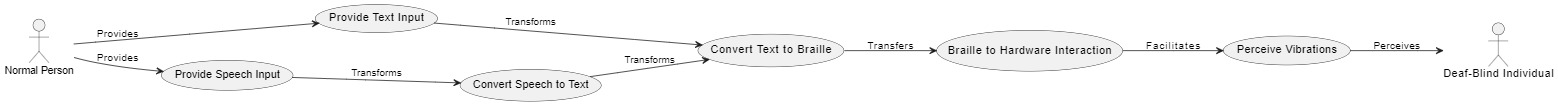
\includegraphics[width=1\textwidth, height=0.2\textwidth]{./pic/UC2.jpg}\\
% \caption{Use case Diagram}
% \end{figure}

% \noindent This use case diagram illustrates the interactions between actors and the system's functionalities in facilitating communication for the deaf-blind community, from input provision by a normal person to the ultimate perception of vibrations by a deaf-blind individual\\\\
% \noindent\textbf{Actors:}\\
% Normal Person: Represents individuals who interact with the system to provide input, either in the form of text or speech.\\
% Deaf-Blind Individual: Represents individuals who are the ultimate recipients of the communication facilitated by the system.\\

% \noindent\textbf{Use Cases:}\\
% Provide Text Input: Use case where the normal person provides input in the form of text to the system.
% \\Provide Speech Input: Use case where the normal person provides input in the form of speech to the system.
% \\Convert Speech to Text: Use case where the system converts the speech input provided by the normal person into text format.
% \\Convert Text to Braille: Use case where the system converts input, whether text provided directly or speech converted to text, into Braille format.
% \\Braille to Hardware Interaction: Use case where the system interacts with Braille hardware to convert Braille output into physical vibrations.
% \\Perceive Vibrations: Use case where the vibrations generated by the hardware are perceived by the deaf-blind individual, facilitating communication.\\

% \noindent\textbf{Actor-Use Case Relationships:}\\
%  Normal Person to Use Cases: The "Normal Person" actor interacts with the system by providing text or speech input, which triggers the corresponding use cases.
% \\Deaf-Blind Individual to Perceive Vibrations Use Case: The "Deaf-Blind Individual" actor perceives the vibrations generated by the hardware, which is represented by the "Perceive Vibrations" use case.\\


% \noindent\textbf{Use Case Relationships:}\\
% Convert Speech to Text to Convert Text to Braille: The "Convert Speech to Text" and "Convert Text to Braille" use cases are connected, indicating that the text output from speech conversion is further processed to convert it into Braille format.
% \\Text Input and Speech Input to Convert Text to Braille: Both "Provide Text Input" and "Provide Speech Input" use cases are connected to "Convert Text to Braille," indicating that regardless of the input method, the system converts it to Braille for further processing.




% \section{Functional Design}
% \subsection{Sequence Diagram}

% \begin{figure}[hbtp]
% \centering

% 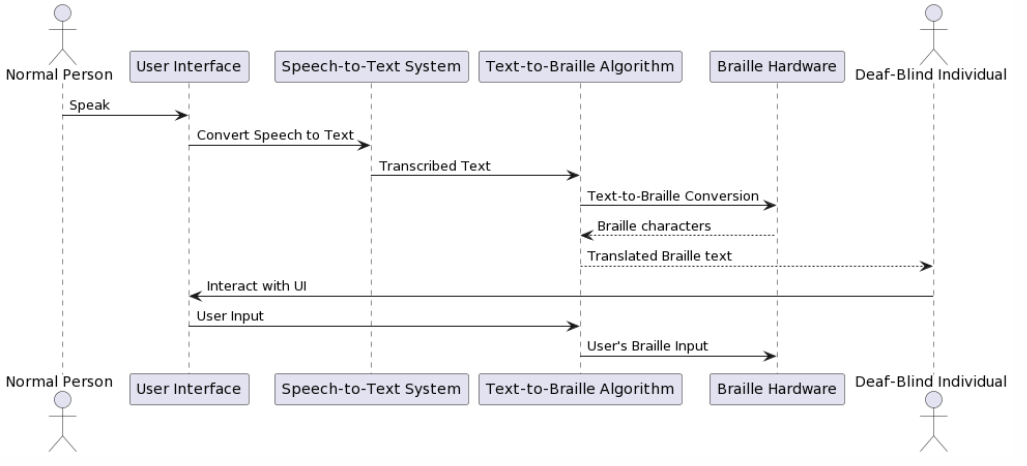
\includegraphics[width=1\textwidth, height=0.6\textwidth]{./pic/seq.png}\\
% \caption{Sequence Diagram}
% \end{figure}

% \noindent\textbf{Normal Person Interaction:}\\
% The communication process commences with the "Normal Person" initiating a conversation by speaking. This reflects the conventional method of conveying information, allowing for natural and spontaneous communication.

% \noindent\textbf{Speech-to-Text Conversion:}\\
% The spoken words are captured by the system's "User Interface," representing the first step in the conversion process. The "User Interface" serves as the gateway for the normal person to interact with the system.
% The speech is then processed by the "Speech-to-Text System," employing robust speech recognition tools or APIs such as Google Cloud Speech-to-Text or Python's SpeechRecognition library. This step ensures the accurate conversion of spoken words into written text.
% The accuracy of speech-to-text conversion is crucial for maintaining the fidelity of the communicated information, enabling precise and meaningful interactions between the normal person and the deaf-blind individual.\\

% \noindent\textbf{Text-to-Braille Conversion:}\\
% The transcribed text undergoes the next transformation through the "Text-to-Braille Algorithm." This sophisticated algorithm is designed to translate the transcribed text into Braille characters, catering to the specific needs of the deaf-blind individual.
% The algorithm supports various Braille standards and languages, ensuring versatility in communication. Additionally, efficiency is prioritized to minimize processing time for text-to-Braille conversion, facilitating a near real-time communication experience.
% This stage in the process is pivotal, as it bridges the gap between the digital representation of text and its tactile counterpart in the form of Braille. The system aims to provide a seamless and efficient means of communication for the deaf-blind individual.\\\\

% \noindent\textbf{Braille Hardware Integration:}\\
% The translated Braille characters are then transmitted to the "Braille Hardware," which constitutes a handheld device containing sensors and actuators. This integration allows for the physical representation of Braille characters, enabling the deaf-blind individual to read and understand the communicated information through tactile feedback.
% Real-time sensory updates from the Braille Hardware ensure a dynamic and responsive interaction experience. This stage emphasizes the tangible aspect of communication, recognizing the importance of tactile feedback for individuals who are both deaf and blind.\\

% \noindent\textbf{Communication to Deaf-Blind Individual:}\\
% The Braille Hardware communicates the translated Braille text directly to the "Deaf-Blind Individual," establishing a direct link between the information conveyed by the normal person and the tactile representation experienced by the deaf-blind individual.
% This direct communication channel ensures that the deaf-blind individual receives the information in a format that is accessible and meaningful, fostering effective communication and understanding.\\

% \noindent\textbf{User Interface Interaction:}\\
% Simultaneously, the deaf-blind individual has the opportunity to interact with the "User Interface." This interaction loop provides a means for the user to actively engage with the system beyond receiving information, contributing to a more participatory communication experience.
% The user interface serves as a central hub for user input, allowing the deaf-blind individual to provide feedback, respond to prompts, or initiate interactions. This bidirectional communication aspect enhances the inclusivity and versatility of the system.


% \section{Access Layer Design}
% \subsection{Dataflow Diagram}

% \begin{figure}[hbtp]
% \centering

% 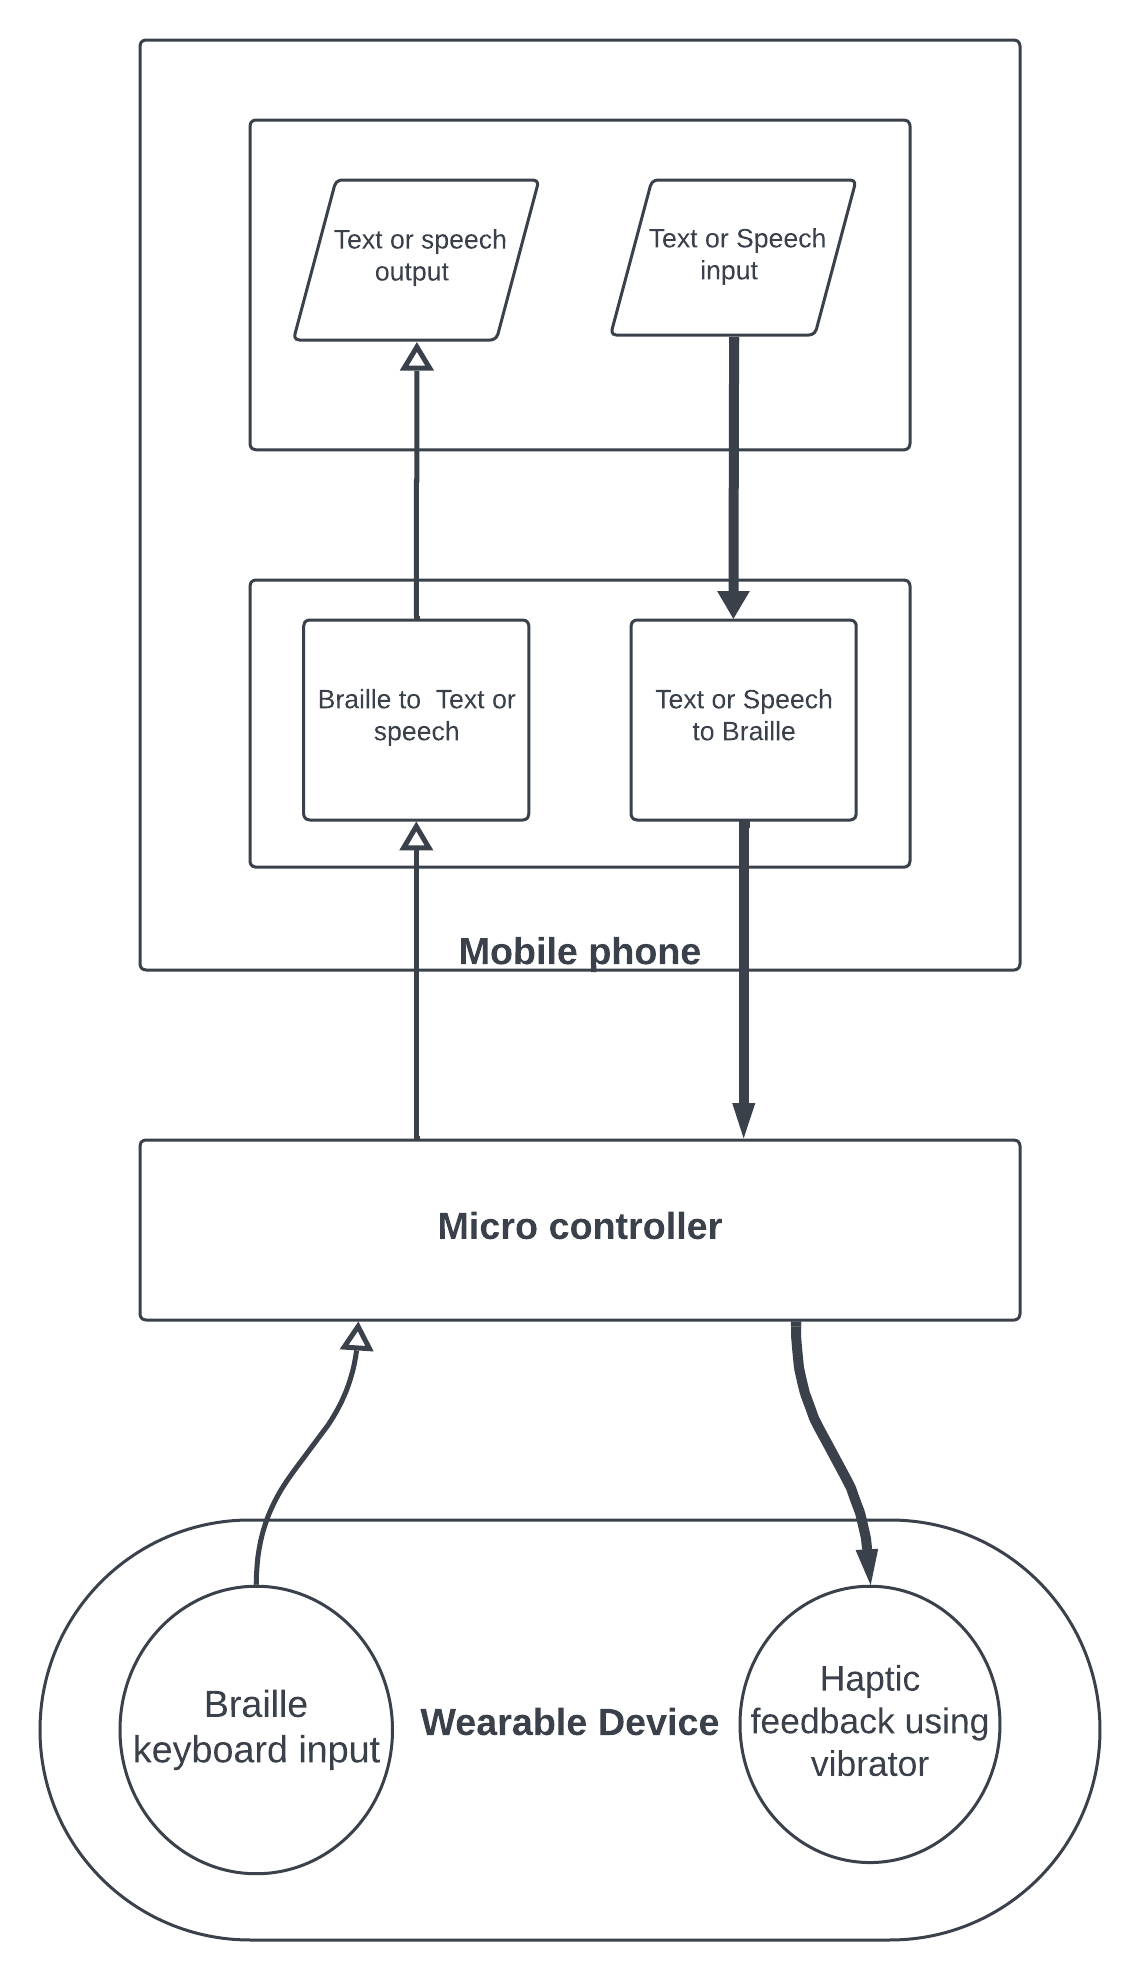
\includegraphics[width=0.7\textwidth, height=1\textwidth]{./pic/dataflow.png}\\
% \caption{Dataflow diagram}
% \end{figure}

% \noindent 
% A Data Flow Diagram (DFD) visually represents the pathway of data within a system, illustrating the flow from textual input by a typical user to haptic output for the deaf-blind individual. Additionally, it portrays the flow from braille input by the deaf-blind individual to textual output for the typical user.\\

% \noindent\textbf{Mobile phone:}\\
% The mobile phone serves as the central platform for executing the software components of the program. It facilitates various essential tasks, such as capturing user input in the form of text or speech, converting this input into braille for tactile feedback, and reciprocally, transforming braille input into textual or audible output. This multifaceted functionality encapsulates the core operations of the program, enabling seamless communication between users with diverse sensory capabilities.\\

% \noindent\textbf{Micro controller:}\\
% The microcontroller component of the system processes braille signals received from the user, interpreting them to activate the appropriate actuators for tactile feedback. Additionally, it collects input from the deaf-blind individual, facilitating communication by sending this data to the mobile phone for processing and interpretation.\\ This microcontroller-mediated exchange ensures efficient interaction between the user and the system, enhancing accessibility for individuals with sensory impairments.\\

% \noindent\textbf{Wearable device:}\\
% The wearable device serves as the primary interface for the deaf-blind individual to interpret incoming braille signals from the phone. Positioned on the palm of the user, it features three actuators on each hand, representing the six dots of braille. These actuators provide tactile feedback, enabling the user to perceive the braille characters through touch.\\
% Beyond tactile feedback, the wearable device also facilitates communication by collecting inputs from the deaf-blind individual. These inputs are then transmitted to the mobile phone for processing and further interaction with the typical user. By bridging the communication gap between the deaf-blind individual and the broader user community, the wearable device enhances accessibility and facilitates meaningful interactions for individuals with sensory impairments.

\chapter{System Design}
This chapter outlines the system design for the Cloud-Based Smart Monitoring System for Baby Health and Safety, detailing the system's architecture, functionality, control flow, access layers, and user interface design. Each section includes design diagrams, descriptions, and an explanation of how they apply to the project.
\section{Abstract Design}

\subsection{Architectural diagram}
The architectural diagram shown in Figure \ref{fig:architecture} represents the high-level structure of the system, illustrating the relationships between various components. The key components of the architecture include IoT sensors for data collection, a Raspberry Pi for data processing, cloud infrastructure for storage, and a mobile application for data access and monitoring.
\begin{itemize}
  \item \textbf{User (Parents):} The caregiver uses the mobile application to initiate data recordings for essential health parameters such as heart rate, temperature, SpO2 levels, and humidity. They receive notifications directly on their mobile device if any abnormal readings or health concerns are detected.
  \item \textbf{Mobile User Interface:} This interface on the caregiver’s mobile device serves as the primary point of interaction, where requests for data are sent to the sensing system and health information is displayed for monitoring.
  \item \textbf{Sensing System:} Comprised of sensors like the Humidity Sensor, Heart Rate Sensor, Temperature Sensor, and SpO2 Sensor, this system captures real-time health data from the baby and forwards it to the processor for further analysis.
  \item \textbf{Processor (Raspberry Pi):} The Raspberry Pi processes the raw data received from the sensors, organizing it into a format suitable for storage and retrieval, and sends it to the Firebase database.
  \item \textbf{Database (Firebase):} The database acts as a central storage location, holding all processed data. It enables the mobile application to retrieve information as needed and supports real-time monitoring by the machine learning model.
  \item \textbf{Pre-trained ML Model:} This model monitors the data in Firebase for any patterns or values that indicate potential health issues. When abnormal readings are detected, it generates alerts that are immediately sent to the caregiver via the mobile app.
\end{itemize}
\begin{figure}[hbtp]
  \centering
  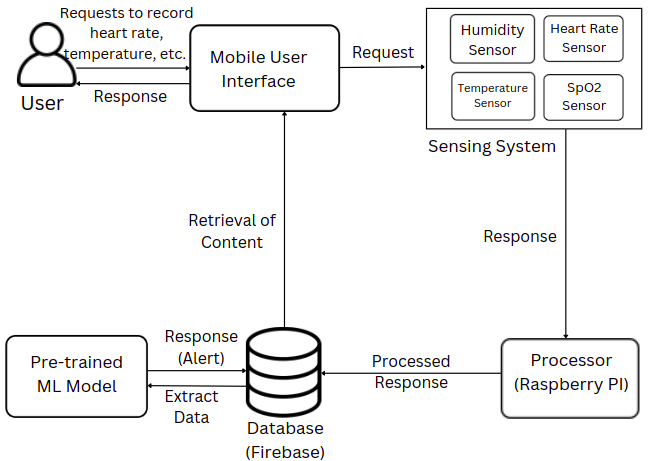
\includegraphics[scale=0.6]{./pic/architecture.png}
  \caption{Architectural Diagram showing the interaction of various entities of the baby monitoring system.}
  \label{fig:architecture}
\end{figure}
\subsection{Use Case Diagram}
The use case diagram shown in Figure \ref{fig:usecase} captures the various interactions between the user and the system, demonstrating how the parent or caregiver interacts with different functionalities to ensure the baby’s safety and well-being. This diagram highlights the key features of the system from a user perspective.
\begin{itemize}
  \item \textbf{Actors:} The primary actor in this system is the parent or caregiver who uses the mobile application to interact with the system. The parent relies on the app to receive real-time data, notifications, and alerts about the baby's status. Secondary actors may include medical professionals or support staff who could access the system during emergencies.
  \item \textbf{Use Cases:} The use cases represent the main functionalities available to the parent. These include:
  \begin{itemize}
    \item \textbf{Monitoring Baby’s Health Metrics:} The system displays real-time information such as the baby's temperature, heart rate, room humidity, and SpO2 levels on the dashboard. This allows parents to continuously keep track of their baby’s well-being from any location.
    \item \textbf{Viewing Live Video Feeds:} Parents can access a live video stream of their baby’s crib or play area. This feature allows for constant visual monitoring, providing additional peace of mind.
    \item \textbf{Receiving Alerts for Abnormal Conditions:} The system triggers alerts if it detects unsafe conditions, such as the baby rolling onto their stomach, abnormal heart rate, or a high room temperature. These notifications are sent instantly to the parent's mobile device.
    \item \textbf{Managing System Settings:} The parent can configure various settings, such as setting thresholds for temperature and heart rate, managing notification preferences, and adjusting video feed quality. The system also allows parents to toggle between real-time data and historical data views.
    \item \textbf{Exporting Historical Data:} Parents can view or export the baby’s historical health data for further analysis or sharing with healthcare professionals. This feature provides a long-term record of the baby’s health trends, which can be helpful for medical consultations.
  \end{itemize}
\end{itemize}
\begin{figure}[hbtp]
  \centering
  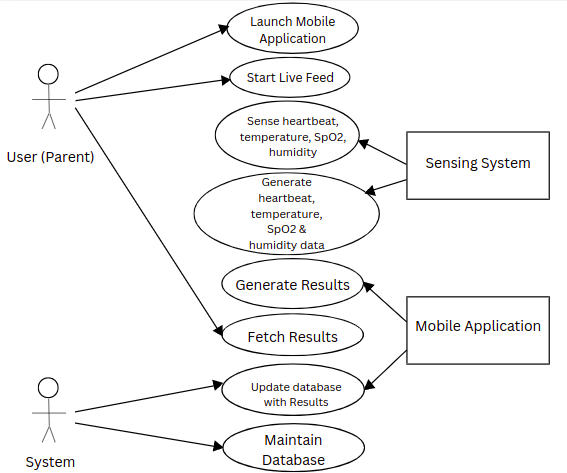
\includegraphics[scale=0.6]{./pic/usercase.png}
  \caption{Use Case Diagram showing the interaction between users and the system.}
  \label{fig:usecase}
\end{figure}
\section{Functional Design}
\subsection{Sequence diagram}
The sequence diagram in Figure \ref{fig:sequence} demonstrates the flow of actions between the User, Mobile Application, Sensing System, and Database in the Cloud-Based Smart Monitoring System for Baby Health and Safety. Here's a detailed breakdown of the steps involved:
\begin{enumerate}
  \item \textbf{User starts the mobile application:} The process begins when the user (typically a parent or caregiver) opens the mobile app to monitor the baby’s health metrics in real-time.
  \item \textbf{User starts the live feed:} Once inside the app, the user initiates the live feed, which triggers the sensing system to collect data from various sensors monitoring the baby’s environment and health.
  \item \textbf{Sensing System collects data:} The sensing system comprises multiple sensors that continuously measure various parameters:
  \begin{itemize}
    \item  \textbf{Heartbeat:} A sensor records the baby’s heart rate.
    \item \textbf{Humidity:} The surrounding room humidity is sensed to ensure it is within a safe range.
    \item \textbf{Temperature:} The baby’s body temperature and room temperature are monitored.
    \item \textbf{SpO2:} A sensor checks the baby’s blood oxygen saturation (SpO2) to track oxygen levels.
  \end{itemize}
  \item \textbf{Data is stored in the Database:} After processing the sensor data, the sensing system sends it to the cloud-based database, where it is stored for real-time analysis and long-term record-keeping.
  \item \textbf{Alert is triggered:} If any of the sensed values exceed predefined safety thresholds (e.g., an abnormal heart rate or high room temperature), an alert is triggered, and the system generates a notification to inform the user.
  \item \textbf{Results are returned to the Mobile Application:} The mobile app retrieves the processed data from the database and displays it in the user interface. The user can then see real-time health metrics and make informed decisions based on the system's results.
  \item \textbf{User views the results:} Finally, the user views the current health metrics and environmental data on the mobile application, ensuring that the baby is in a safe and healthy condition. If an alert was triggered, the user will also be notified within the app.
\end{enumerate}
\begin{figure}[hbtp]
  \centering
  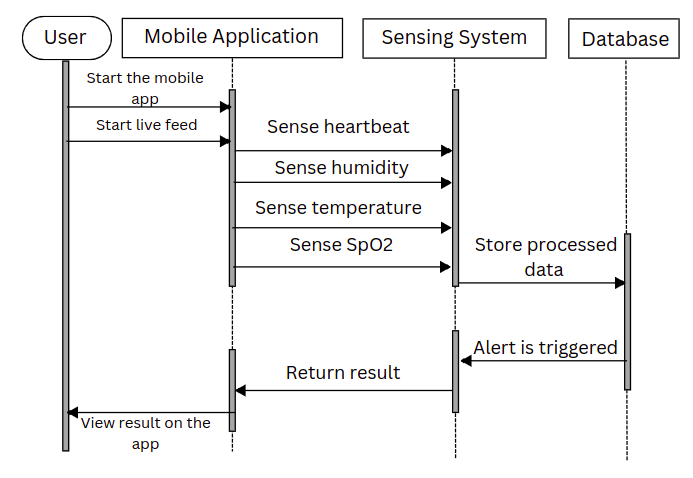
\includegraphics[scale=0.6]{./pic/sequence.png}
  \caption{Sequence diagram showing the timeline of interaction between different entities in the system}
  \label{fig:sequence}
\end{figure}

\section{Access Layer Design}
\subsection{Data Flow Diagram}
The data flow diagram shown in Figure \ref{fig:dataflow} outlines how data travels through the system, highlighting the interaction between sensors, the Raspberry Pi, cloud storage, and the mobile application.
\begin{itemize}
  \item \textbf{Sensors:} The first layer involves IoT sensors collecting real-time data on the baby’s health and environmental conditions.
  \item \textbf{Raspberry Pi:} The Raspberry Pi acts as a bridge, processing sensor data and relaying it to the cloud.
  \item \textbf{Cloud Database:} In the cloud, data is securely stored and processed. The system continuously checks the data against preset safety thresholds and sends alerts when abnormalities are detected.
  \item \textbf{Mobile Application:} The app fetches data from the cloud and displays it to the user in real-time. Parents can also retrieve historical data for deeper insights into the baby’s health trends.
\end{itemize}
\begin{figure}[hbtp]
  \centering
  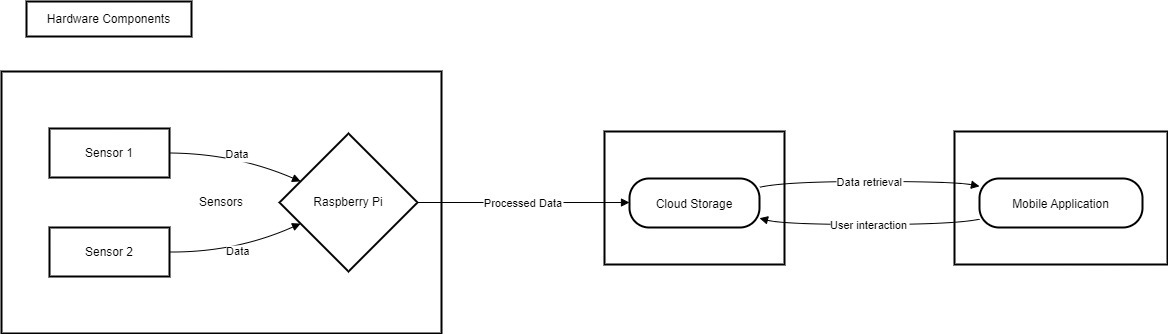
\includegraphics[scale=0.35]{./pic/WhatsApp Image 2024-10-23 at 22.00.55_66baa9c8.jpg}
  \caption{Data flow diagram showing how the data travels through the system}
  \label{fig:dataflow}
\end{figure}

\section{Presentation Layer Design}
\subsection{User Interface Flow Design}
The user interface flow for the application (Figure \ref{fig:uiflow}) is designed to provide parents with an intuitive and seamless experience for monitoring their baby's health and environment. The following steps describe the flow from the onboarding process to the profile management:
\begin{enumerate}
  \item \textbf{Onboarding Screen:} Upon launching the app, the user is welcomed with the onboarding screen, which introduces the app’s primary function, ensuring peace of mind for every parent by offering baby health monitoring in the palm of their hand. This screen includes an image carousel showcasing key features like monitoring baby movements, temperature, humidity, and more. The user is prompted to continue with email to proceed further.
  \item \textbf{Sign-Up Screen:} New users are taken to the Sign-Up screen after the onboarding. Here, they can create an account by providing a username, email, and password. A simple and user-friendly form guides the registration process. After filling in the details, they can tap Sign Up. If they already have an account, they are given the option to switch to the login screen.
  \item \textbf{Login Screen:} Existing users access the Login screen, where they can sign in by entering their email and password. There’s also a Forgot password option for those who might need help recovering their credentials. After entering valid credentials, the user taps Log In to access the app’s features.
  \item \textbf{Home Screen:} After logging in, the user is taken to the Home screen. This screen displays key baby health data, including real-time temperature tracking, humidity levels and SpO2 levels.
  \item \textbf{Stats Screen:} The Stats screen gives a detailed view of the baby’s health trends over time. 
  \item \textbf{Profile Screen:} The Profile screen offers personalized features for the user. They can call a doctor directly from the app if any issues are detected, access emergency contacts quickly for immediate assistance, modify details such as contact information, health preferences, and other personal settings to ensure the app is tailored to their needs.
\end{enumerate}
\begin{figure}[hbtp]
  \centering
  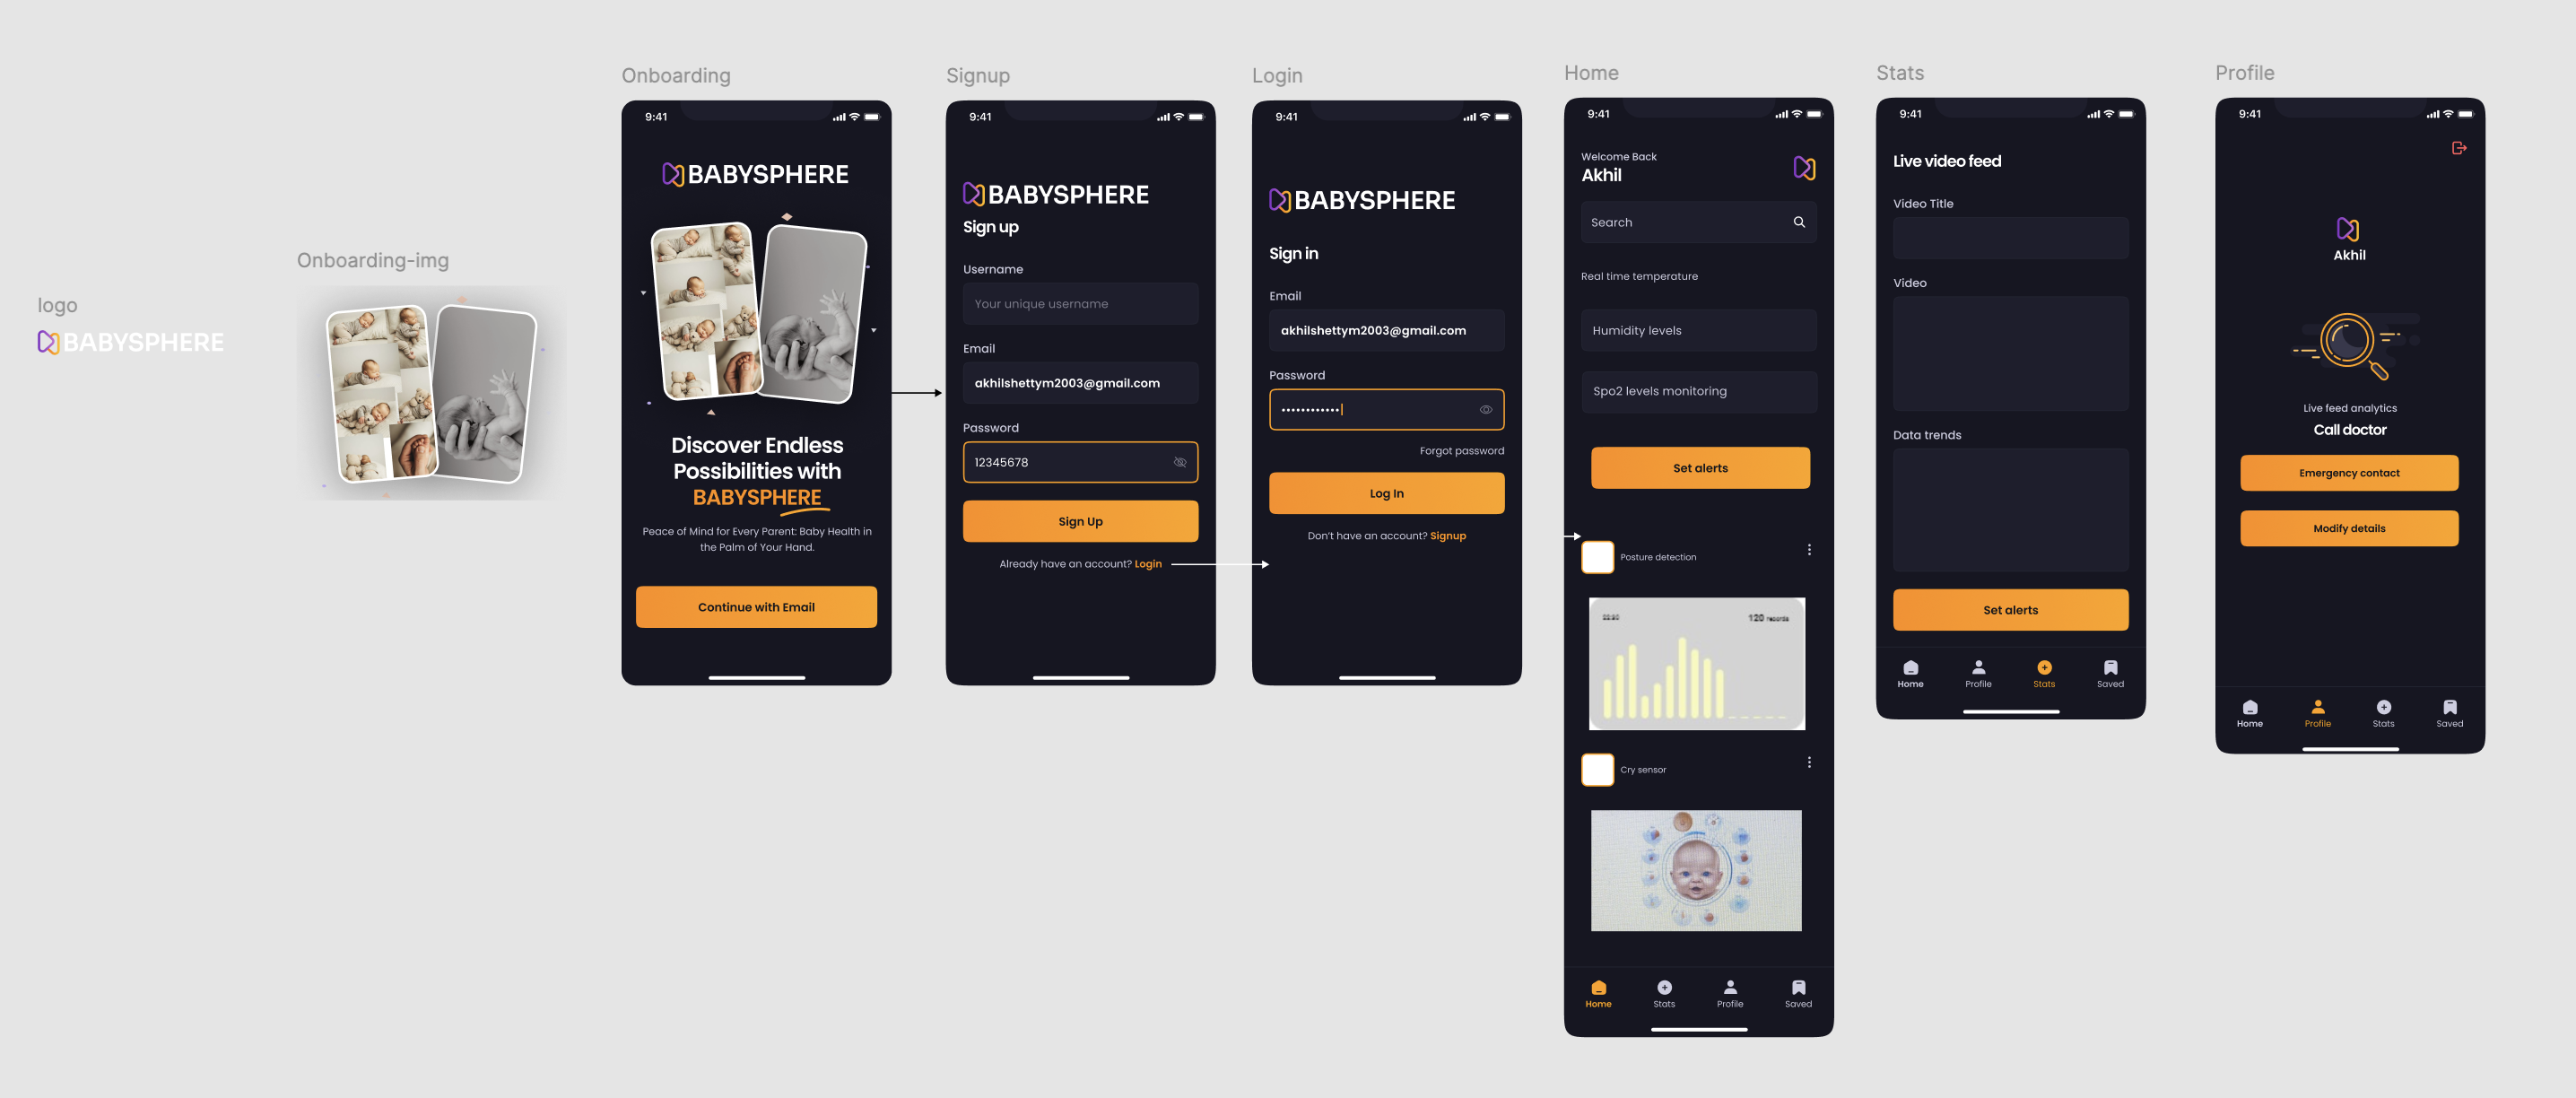
\includegraphics[scale=0.32]{./pic/uiflow.png}
  \caption{User Interface Flow Design of the mobile app designed using Figma}
  \label{fig:uiflow}
\end{figure}
\newpage
\renewcommand{\bibname}{References}

\addcontentsline{toc}{chapter}{References}
% \begin{thebibliography}{35}
%   \bibitem{ref1}
%   Ramirez-Garibay, F., Olivarria, C. M., Eufracio Aguilera, A. F., and Huegel, J. C. (2014). MyVox—Device for the communication between people: blind, deaf, deaf-blind and unimpaired. IEEE Global Humanitarian Technology Conference (GHTC 2014), 12, 506–509. https://doi.org/10.1109/ghtc.2014.6970330


%   \bibitem{ref2}
%   Ulrike Gollner, Tom Bieling, and Gesche Joost. 2012. Mobile Lorm Glove: introducing a communication device for deaf-blind people. In Proceedings of the Sixth International Conference on Tangible, Embedded and Embodied Interaction (TEI '12). Association for Computing Machinery, New York, NY, USA, 127–130. https://doi.org/10.1145/2148131.2148159

%   \bibitem{ref3}
%   Arthur Theil, Lea Buchweitz, James Gay, Eva Lindell, Li Guo, Nils-Krister Persson, and Oliver Korn. 2020. Tactile Board: A Multimodal Augmentative and Alternative Communication Device for Individuals with Deafblindness. In Proceedings of the 19th International Conference on Mobile and Ubiquitous Multimedia (MUM '20). Association for Computing Machinery, New York, NY, USA, 223–228. https://doi.org/10.1145/3428361.3428465

%   \bibitem{ref4}
%   Narute, P., Pote, A., Poman, A., and Pawar, S. (2018). An efficient communication system for blind, dumb and deaf people. International Research Journal of Engineering and Technology (IRJET), 5(1), 1561-1563.

%   \bibitem{ref5}
%   Evreinova, T., Evreinov, G., and Raisamo, R. (2002). Communication system for the people who are deaf or have low vision. In Proceedings of HANDICAP 2002 2ème Conférence pour l'essor des technologies d'assistance (pp. 115-120)

%   \bibitem{ref6}
%   Ghorpade, S. R., and Waghmare, S. K. (2015). A Communication System for Deaf and Dumb People. Hand, 1, 2.

%   \bibitem{ref7}
%   Monti, L., and Delnevo, G. (2018). On improving GlovePi: Towards a many-to-many communication among deaf-blind users. 2018 15th IEEE Annual Consumer Communications \&amp; Networking Conference (CCNC), 9, 1–5. https://doi.org/10.1109/ccnc.2018.8319236

%   \bibitem{ref8}
%   Duvernoy, B., Kappassov, Z., Topp, S., Milroy, J., Xiao, S., Lacôte, I., Abdikarimov, A., Hayward, V., and Ziat, M. (2023). HaptiComm: A Touch-Mediated Communication Device for Deafblind Individuals. IEEE Robotics and Automation Letters, 8(4), 2014–2021. https://doi.org/10.1109/lra.2023.3241758023, doi: 10.1109/LRA.2023.3241758.
% \end{thebibliography}
\printbibliography

\end{document}